\documentclass[11pt]{article}
\setlength{\parindent}{0pt}
\usepackage{xltxtra}
\usepackage{hyperref}
\hypersetup{hidelinks}
\usepackage{url}
\urlstyle{tt}
\usepackage{xcolor}
\definecolor{CVBlue}{RGB}{23,110,191}
\usepackage{calc}
\usepackage{graphicx}
\usepackage{tikz}
\usetikzlibrary{calc}
\usepackage{fontspec}
\usepackage{xeCJK}
\usepackage{enumitem}
\CJKsetecglue{}
\setmainfont[
Path = fonts/Main/,
Extension = .otf,
BoldFont = texgyretermes-bold.otf,
]{texgyretermes-regular.otf}
\setCJKmainfont[
Path = fonts/hansans/,
Extension = .ttf,
BoldFont = NotoSansSC-Bold.ttf,
]{NotoSansSC-Regular.otf}
\usepackage{relsize}
\usepackage{xspace}
\usepackage{fontawesome}
\usepackage[
a4paper,
left=1.2cm,
right=1.2cm,
top=1.5cm,
bottom=1cm,
nohead
]{geometry}
\renewcommand{\baselinestretch}{1.5}
\usepackage{titlesec}
\usepackage{enumitem}
\setlist{noitemsep}
\setlist[itemize]{topsep=0.25em, leftmargin=*}
\setlist[enumerate]{topsep=0.25em, leftmargin=*}
\newlength{\interProjectSpacing}
\setlength{\interProjectSpacing}{0.9em}
\newcommand{\projectsep}{\vspace{\interProjectSpacing}}
\newlength{\intraProjectTitleSep}
\setlength{\intraProjectTitleSep}{0.4em}
\newcommand{\titlebreak}{\\[\intraProjectTitleSep]}
\newlength{\intraProjectListTopSep}
\setlength{\intraProjectListTopSep}{0.2em}
\titleformat{\section}
{\large\bfseries\raggedright}
{}{0em}
{}
[{\color{CVBlue}\titlerule}]
\titlespacing*{\section}{0cm}{*1.6}{*1.2}

\begin{document}
\pagenumbering{gobble}
\begin{tikzpicture}[remember picture, overlay]
\node[anchor = north east] at ($(current page.north east)+(-2.0 cm,-0.3cm)$) {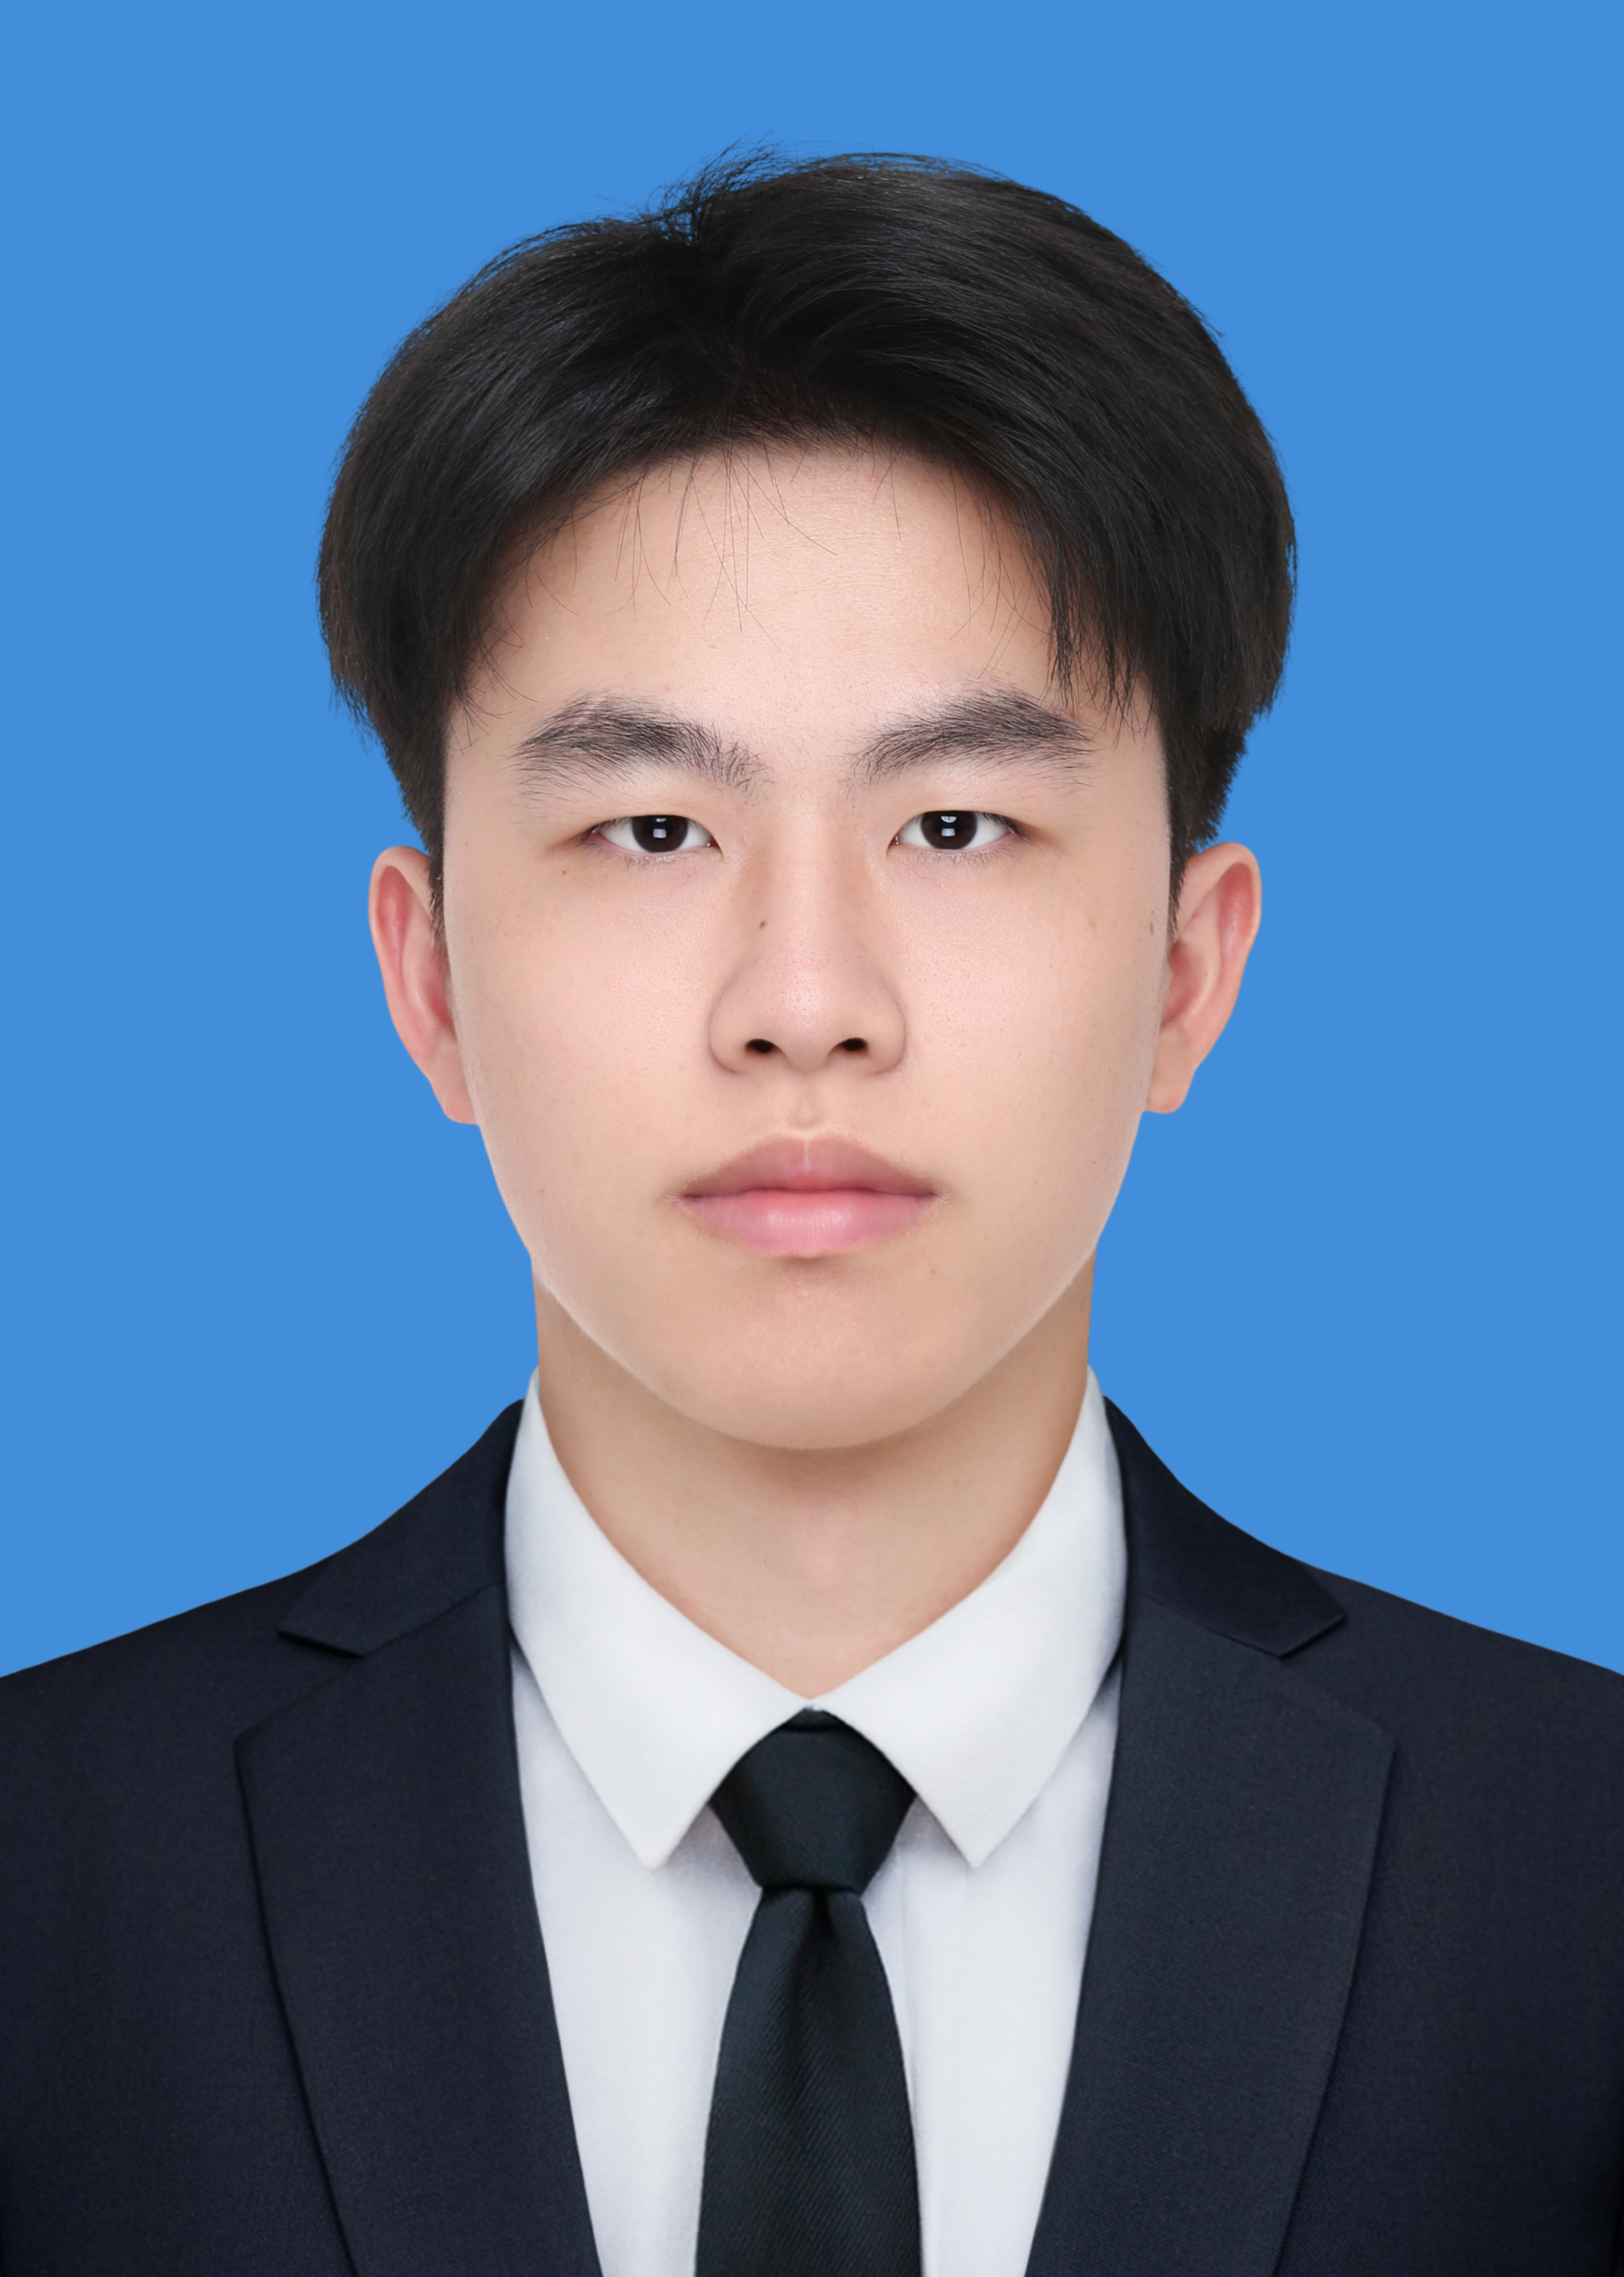
\includegraphics[height=3cm]{yxl.jpg}};
\end{tikzpicture}%
\begin{tikzpicture}[remember picture, overlay]
\node[anchor = north west] at ($(current page.north west)+(0.5cm,+1.0cm)$) {\includegraphics[height=6cm]{zju.png}};
\end{tikzpicture}%
\centerline{\LARGE\bfseries{杨仙林}}
\centerline{\normalsize{\faPhone\ 15828872384 \quad \faEnvelopeO\ \href{mailto:1295510209\@qq.com}{1295510209\@qq.com}}}
\section{\makebox[\widthof{\faGraduationCap}][c]{\color{CVBlue}\faGraduationCap}\ 教育背景}
\textbf{浙江大学} \hfill \\[0.5em]
本科 \quad 控制科学与工程学院 \quad 自动化  \quad 2020.9-2024.6
\\[0.5em]
硕士 \quad 工程师学院 \quad 控制工程  \quad 2024.9-至今
\section{\makebox[\widthof{\faCogs}][c]{\color{CVBlue}\faCogs}\ 专业技能}
\begin{itemize}[nosep]
\item \textbf{编程语言：} Python、C
\item \textbf{算法方向：} 深度学习、目标检测、时序预测、故障诊断
\item \textbf{英语能力：} CET-6
\end{itemize}
\section{\makebox[\widthof{\faTrophy}][c]{\color{CVBlue}\faTrophy}\ 荣誉奖项}
\begin{itemize}[nosep]
\item 2025 浙江大学二等学业优秀奖助金
\item 2023 浙江大学力悦创投奖学金
\item 2023 浙江省大学生数学竞赛三等奖
\end{itemize}
\section{\makebox[\widthof{\faBook}][c]{\color{CVBlue}\faBook}\ 科研成果}
\begin{itemize}[nosep]
\item 2025.07 中国过程控制会议论文：《PatchX-MLP: 一种用于 SCR 入口 NOx 浓度预测的时序预测算法》
\end{itemize}
\section{\makebox[\widthof{\faUsers}][c]{\color{CVBlue}\faUsers}\ 项目经历}
\projectsep
\textbf{基于 PatchX-MLP 的 SCR 入口 NOx 浓度预测} \hfill 2025.03 -- 2025.08 \titlebreak
\begin{itemize}[nosep, topsep=\intraProjectListTopSep]
\item \textbf{项目简介：} 面向 SCR 入口 NOx 浓度预测，融合多变量运行数据，建模工况变化与时序依赖，为脱硝过程运行优化提供预测依据。
\item \textbf{技术栈：} Python、PyTorch、MLP、多尺度 Patch、时序分解、时频域联合损失
\item \textbf{模型设计：} 采用多尺度 Patch 分割及趋势与季节项分解，通过 MLP 在 Patch 内、Patch 间及变量间建立交互，实现局部变化、长期趋势与变量关联的多特征融合。
\item \textbf{训练与验证：} 完成时域误差与频域约束的联合优化及消融实验；工业数据 96 步预测的 MSE / MAE 为 0.228 / 0.223，较 TimeMixer 分别降低 6.6\% / 5.5\%。
\end{itemize}

\projectsep
\textbf{大模型话题与安全检测系统} \hfill 2026.06 -- 2026.08 \titlebreak
\begin{itemize}[nosep, topsep=\intraProjectListTopSep]
\item \textbf{项目简介：} 面向 LLM 应用搭建可配置的请求检测模块，识别业务话题、提示词攻击和有害内容，为模型调用提供风险判断与路由依据。
\item \textbf{技术栈：} Python、PyTorch、Transformers、预训练编码器、多任务学习、FastAPI
\item \textbf{检测建模：} 以预训练文本编码器提取语义特征，配置话题、攻击与有害内容分类头；通过掩码损失利用不同来源数据的部分标签，支持检测任务扩展与底层模型替换。
\item \textbf{数据与策略：} 完成数据清洗、去重及训练、校准、测试集拆分；按误报约束校准阈值，结合话题白名单与风险得分，设计放行、拒答和复核三类决策。
\item \textbf{工程实现：} 封装训练、评估与推理流程，提供检测接口及类别、分数和触发原因；对低置信度或检测能力缺失的请求设置复核分支，便于接入上层应用。
\end{itemize}

\projectsep
\textbf{基于大模型的工作票智能生成系统} \hfill 2025.09 -- 2026.09 \titlebreak
\begin{itemize}[nosep, topsep=\intraProjectListTopSep]
\item \textbf{项目简介：} 面向电气检修任务，基于 Dify 搭建 Agent 框架，编排图纸解析、知识检索、内容生成与校验流程，辅助生成工作票中的工作内容与安全措施。
\item \textbf{技术栈：} Dify、LLM Agent、Tool Calling、VL Embedding、SAM、GraphRAG、Python
\item \textbf{图纸抽取：} 利用大模型视觉特征匹配图例与多尺度图块，定位设备候选区域，再以 SAM 细化分割边界；结合 OCR 与位置约束关联设备编号，输出设备类别、位置及标识等结构化信息。
\item \textbf{图谱检索：} 设计设备、检修任务、安规条款与历史工作票的关联检索流程；结合 GraphRAG 的实体关系检索与文本语义召回，组织相关条款及历史案例，并保留来源证据供生成与核验使用。
\item \textbf{Agent 编排：} 将图纸抽取与检索能力封装为可调用工具，通过工作流传递检修范围、设备信息和证据；结合 Prompt 与结构化模板生成票面内容，设置必填项、设备一致性检查及人工复核环节。
\item \textbf{SFT 适配方案：} 设计基于历史工作票的指令样本与 LoRA 微调方案，以“检修任务＋检索证据”为输入、票面字段为输出，规划术语一致性、字段完整性与证据符合性评估，强化领域表达和格式遵循。
\end{itemize}

\end{document}
